\documentclass[10pt,a4paper]{article}

% USE NORMAL DATES
\usepackage{datetime}

% GRAPHICS
%\usepackage{graphicx}

% FONTS for pdfLaTeX
%\usepackage[charter]{mathdesign}
%\usepackage[scaled=0.86]{berasans} % sans-serif font
%\usepackage{inconsolata} % typewriter
%\usepackage[T1]{fontenc}

% FONTS for XeLaTeX
\usepackage{fontspec}
\setmainfont[Scale=1.1]{Cambria}
\setsansfont{Tahoma}
\setmonofont{Consolas}
%\usepackage{unicode-math}
%\setmathfont{Cambria Math}

% SECTION FONT STYLE
\usepackage{sectsty}
\allsectionsfont{\sffamily} % make sections sans-serif

% PAGE BORDERS
\usepackage[top=40mm,bottom=20mm,left=25mm,right=25mm]{geometry}

% PARAGRAPH BEHAVIOUR
\setlength{\parskip}{1em}
\setlength{\parindent}{0pt}

% CODE FORMATTING
\usepackage{listings}
\usepackage[usenames,dvipsnames]{color}
\definecolor{LightGray}{rgb}{0.95,0.95,0.95}

\lstdefinestyle{myC}{
  belowcaptionskip=1\baselineskip,
  breaklines=true,
  backgroundcolor=\color{LightGray},
  frame=none,
  numbers=none,
  numbersep=10pt,
  numberstyle=\color{Gray},
  xleftmargin=10pt,
  language=C,
  showstringspaces=false,
  basicstyle=\small\ttfamily,
  keywordstyle=\bfseries\color{Blue},
  commentstyle=\itshape\color{ForestGreen},
  identifierstyle=\color{Fuchsia},
  stringstyle=\color{Sepia},
}

\lstdefinestyle{myPascal}{
  belowcaptionskip=1\baselineskip,
  breaklines=true,
  backgroundcolor=\color{LightGray},
  frame=none,
  numbers=none,
  numbersep=10pt,
  tabsize=2,
  numberstyle=\color{Gray},
  xleftmargin=10pt,
  language=Pascal,
  showstringspaces=false,
  basicstyle=\small\ttfamily,
  comment=[l]{//},
  keywordstyle=\bfseries\color{Blue},
  commentstyle=\itshape\color{ForestGreen},
  identifierstyle=\color{Blue},
  stringstyle=\color{Sepia},
}

\lstdefinestyle{myBash}{
  breaklines=false,
  backgroundcolor=\color{White},
  frame=none,
  numbers=none,
  numbersep=10pt,
  xleftmargin=10pt,
  language=Bash,
  showstringspaces=false,
  basicstyle=\small\ttfamily,
  keywordstyle=\bfseries,
  commentstyle=\itshape,
  identifierstyle=\color{Magenta},
  stringstyle=\color{Sepia},
}


% TITLE PAGE
\title{Creating Pascal bindings for C\\
\vspace{0.5em}
\normalsize v1.0}
\author{W Hunter}
\newdateformat{mydate}{\monthname[\THEMONTH] \THEYEAR}
\date{\mydate\today}

% HYPERLINKS
\usepackage[pdfauthor={William Hunter},
colorlinks=true,
linkcolor=BlueViolet]{hyperref}

% NEW COMMANDS
\newcommand{\mytext}[1]{\textcolor{ForestGreen}{\texttt{#1}}}


% BEGIN DOCUMENT
\begin{document}
\maketitle
\tableofcontents
\clearpage

\section{Purpose of document}
The purpose of this document is to show how to use C libraries from Object
Pascal, more specifically using Free Pascal (FPC). It is inspired by
\cite{cinfree}, but showing a more up to date approach as per
the \textit{Free Pascal Programmer's Guide}
\mytext{http://www.freepascal.org/docs-html/prog/progse28.html},
and with help from `Thaddy' on the FPC forum.

I suggest you read everything in this document (that means the whole
document), including the source files,
because I've also put explanations and hints in them.

In all the examples that follow I'll first show the C code and how to compile it,
and then the same for the Pascal code. Each example has three C source code files: a Header, 
a Module and finally the C program itself.\footnote{If you
want to read up about C programming, have a look at the \textit{Deitel} books on C 
programming, I've also found \textit{C for Linux Programming} (by Castro Lopo, Aitken and 
Jones) to be a good book, especially if you're
going to be using \textit{gcc}.}

If you're not familiar with C you might wonder why one would go through all the
trouble of creating three separate files, especially for something as trivial
as adding two numbers?

One reason is to keep the function definition separate from the actual C program, this way 
you can have many different C programs that can use the same functions (and possibly other 
things). If a function is defined in a C program and you wanted to use it in another 
program, you'd have to rewrite (or copy) that piece of code every time. But you probably 
know this.

Another reason, and relevant in the context of this document, is that C libraries generally 
take this form, namely, they consist of a Header file
and the Module; the examples in this document tries to mimic that.

The approach is one of the following methods:
\begin{enumerate}
\item Compile the C module into an object file (*.o file) and link to the object file, or
\item Create a library (static) from the object files and then link
to the library or
\item Create a library (shared) from the object files and then link
to the library.
\end{enumerate}

I'll show how to do all three methods.

\section{Prerequisites}
You need to have a fairly good knowledge of the C language, and of course of
Object Pascal too. Where I refer to Pascal in this document, it also means
Object Pascal, although in the context of this document it makes little or no difference.

If you spot an error or a typo or an improvement (I'm a hobbyist programmer),
please let me know. You can mail me at \mytext{whunter.za+pbc@NOSPAMgmail.com}
(delete the \mytext{NOSPAM} bit).

\section{Development environments}
\subsection{Windows 7/8.1/10}
You'll need the following two compilers:
\begin{itemize}
\item FPC (Free Pascal Compiler) -- \mytext{http://www.freepascal.org/}
\item GCC (MinGW GNU C Compiler) -- \mytext{http://www.mingw.org/}
\end{itemize}

Setting up MinGW (Minimalist GNU for Windows) on Windows can be painful (to say the least). 
If on 64-bit, I suggest you download \mytext{mingw-w64-install.exe} instead of 
\mytext{mingw-get-setup.exe}, the latter didn't work for me on \textit{Windows 10}.

\subsection{Linux (Ubuntu)}
All the code in this document was compiled and ran successfully in \textit{Ubuntu 14.04 
LTS 64-bit}, using FPC and GCC. The approach on Linux is a little different for Shared 
Objects (Dynamic Libraries) compared to Windows, in particular,
you may have to do the following or a variant thereof:

The C modules must be
compiled as ``position-independent code'' using gcc's `fPIC' flag, for example:

\mytext{gcc -c -fPIC -o sum.o sum.c}\\
\mytext{gcc -c -fPIC -o hello.o hello.c}\\

Create a Shared Object\\
\mytext{gcc -shared -fPIC sum.o hello.o -o liball.so}\\

Set permissions (if required)\\
\mytext{chmod 755 liball.so}

Copy lib to a standard location\\
\mytext{sudo cp liball.so /usr/local/lib/}

Copy headers to a standard location\\
\mytext{sudo cp sum.h /usr/local/include/}
\mytext{sudo cp hello.h /usr/local/include/}

We need to copy the header files to the same location as the library
so that function prototypes are available to someone
who wants to link to the library, unless the prototypes are known otherwise.

Ask loader to update cache\\
\mytext{sudo ldconfig}

\clearpage
\subsection{Compiler versions}
The code examples in this document was last tested and worked on
\textit{Windows 10 64-bit}, using
\begin{itemize}
\item \mytext{Free Pascal Compiler version 3.0.0 [2015/11/16] for i386}
\item \mytext{gcc (x86\_64-win32-seh, Built by MinGW-W64 project) 6.1.0}
\end{itemize}

\subsection{Conventions}
Both Pascal programs and units uses the `pas' file extension.
If using the \textit{Lazarus IDE} to compile your files, you may want to use `lpr' for your
Pascal source files (but apparently not for units).

Static Libraries uses the `a' file extension (referring to the fact that
they're merely archives).

Shared Objects (*.so) and Dynamic Libraries (*.dll) refer to the same thing, although I
read somewhere that it's not a bad idea to keep the `so' extension on Windows machines
too if using \textit{gcc}. That way users know that the library was probably compiled using
\textit{MinGW} tools.

You should know that Pascal code is not case sensitive, but C is, so keep this in
mind when linking to external code, since your function prototypes have to
be \textit{identical}.
\clearpage

\section{Linking to Object files}
\subsection{The sum of two numbers}
A trivial example showing how to calculate the sum of two integer numbers and print the result to standard output.

\subsubsection{C source files}
\lstset{style=myC}
\subsubsection*{Header file 'sum.h'}
This really just contains the function prototype, the rest is a C  ``include guard'' (see for example \newline
\url{http://en.wikipedia.org/wiki/Include\_guard)})

\lstinputlisting{../sum/sum.h}

\subsubsection*{Module 'sum.c'}
This is where the actual function's workings are defined, the function
needs to correspond to the prototype in the Header file.
\lstinputlisting{../sum/sum.c}

\newpage
\subsubsection*{Program 'main1.c'}
Note that in the program we only include the Header file, and then simply call the function. We don't actually need to know how the function is implemented, we just need to know what the function definition looks like (by inspecting the Header file) so that we can use it.

\lstinputlisting{../sum/main1.c}

\subsubsection*{Compiling the C code}
First create an object-code file from the C module; in a terminal (for example, \mytext{ConsoleZ} on \mytext{Windows}) type:

\lstset{style=myBash}
\begin{lstlisting}
gcc -c sum.c
\end{lstlisting}

This should produce an object-code file \mytext{sum.o}. Now create a
program called \mytext{main1.exe} by compiling and linking the
object-code file and creating an executable:

\lstset{style=myBash}
\begin{lstlisting}
gcc sum.o main1.c -o main1.exe
\end{lstlisting}

This should produce a file \mytext{main1.exe} (the 'exe' extension is only required on \mytext{Windows} machines). If you run the program
(by typing its name in the terminal), you should get:

\lstset{style=myBash}
\begin{lstlisting}
From C: The sum of 17 and 19 is 36
\end{lstlisting}
That just proves that the C code compiled and works as expected, which is
obviously important.
\clearpage


\subsubsection{Pascal source files}
Two files are required, namely a Pascal unit and the Pascal program.
\lstset{style=myPascal}

\subsubsection*{Unit 'unit1.pas'}
We link to the C object file via the following Pascal unit.
\lstinputlisting{../sum/unit1.pas}

\subsubsection*{Program 'prog1.pas'}
\lstinputlisting{../sum/prog1.pas}

\textbf{NOTE:-} Nowhere in the above Pascal code did we define how to add two integers (since that would be pointless as it's already defined in the C code).
\clearpage

\subsubsection*{Compiling the Pascal code}
We can now call the ``C generated'' \mytext{sum.o} object file from Pascal code. As you can see from the Pascal code above, the \mytext{sum} function isn't defined anywhere \textbf{except} in the C source code. And that's the whole idea, the intention is to use the ``C generated'' object-file from Pascal and not having to define (write the code for) the function again because it's already been done in C.

Compile the Pascal program (output the file as \mytext{prog1.exe}, \mytext{fpc} will compile and link the files):

\mytext{fpc prog1.pas -oprog1.exe}

If you're on a 64-bit machine, you may have to type this instead (\textbf{this is
true for the rest of the examples too}):

\mytext{fpc -Px86\_64 prog1.pas -oprog1.exe}

This should produce a file \mytext{prog1.exe}. If you run the program (by typing its name in the terminal), you will get

\mytext{From Pascal: The sum of 12 and 51 is 63}.

\textbf{NOTE:-} Since we've passed different values (12 and 51) to the \mytext{sum} function in the Pascal code, we obviously expect a different answer.
\clearpage


\subsection{Printing to screen}
A slightly more complicated example showing how to print to standard output.

For this example to work I had to link to \mytext{libmsvcrt.a} in my MinGW
 directory (just search for it). I just copied the library file to the same
  directory as my source files.

\subsubsection{C source files}
\lstset{style=myC}

\subsubsection*{Header file 'hello.h'}
\lstinputlisting{../hello/hello.h}

\subsubsection*{Module 'hello.c'}
\lstinputlisting{../hello/hello.c}

\newpage
\subsubsection*{Program 'main2.c'}
\lstinputlisting{../hello/main2.c}

\subsubsection*{Compiling the C code}
As before, first create an object-code file from the C module; in a terminal  type:

\lstset{style=myBash}
\begin{lstlisting}
gcc -c hello.c
\end{lstlisting}

This should produce an object-code file \mytext{hello.o}. Now create a
program called \mytext{main2.exe} by compiling and linking the
object-code file and creating an executable:

\lstset{style=myBash}
\begin{lstlisting}
gcc main2.c hello.o -o main2.exe
\end{lstlisting}

This should produce a file \mytext{main2.exe}. If you run the program (by typing its name in a terminal), you will get:

\lstset{style=myBash}
\begin{lstlisting}
From C:
Hello, World!
Hello John Smith
\end{lstlisting}
\clearpage


\subsubsection{Pascal source files}
\lstset{style=myPascal}

\subsubsection*{Unit 'unit2.pas'}
We link to the C object file via the following Pascal unit.
\lstinputlisting{../hello/unit2.pas}

\subsubsection*{Program 'prog2.pas'}
\lstinputlisting{../hello/prog2.pas}

\newpage
\subsubsection*{Compiling the Pascal code}
Compile the Pascal program (output the file as \mytext{prog2.exe}):

\mytext{fpc -Px86\_64 prog2.pas -oprog2.exe}

This should produce a file \mytext{prog2.exe}. If you run the program (by typing its name in the terminal), you will get

\lstset{style=myBash}
\begin{lstlisting}
From Pascal, calling C functions:
Hello, World!
Hello Joe Public
\end{lstlisting}
\clearpage

\subsection{Simple array functions}\label{arrfun}
An example showing how to work with 1-d arrays (vectors)using
\textbf{fun}ctions that operate on \textbf{arr}ays.
\subsubsection{C source files}
\lstset{style=myC}

\subsubsection*{Header file 'arrfun.h'}
\lstinputlisting{../arrfun/arrfun.h}

\subsubsection*{Module 'arrfun.c'}
\lstinputlisting{../arrfun/arrfun.c}

\subsubsection*{Program 'main3.c'}
\lstinputlisting{../arrfun/main3.c}

\clearpage
\subsubsection*{Compiling the C code}
As before, first create an object-code file from the C module; in a terminal  type:

\lstset{style=myBash}
\begin{lstlisting}
gcc -c arrfun.c
\end{lstlisting}

This should produce an object-code file \mytext{arrfun.o}. Now create a
program called \mytext{main3.exe} by compiling and linking the
object-code file and creating an executable:

\lstset{style=myBash}
\begin{lstlisting}
gcc main3.c arrfun.o -o main3.exe
\end{lstlisting}

This should produce a file \mytext{main3.exe}. If you run the program (by typing its name in a terminal), you will get:

\lstset{style=myBash}
\begin{lstlisting}
From C: The multiplied elements are:
Item 0: 6.000000
Item 1: 4.000000
Item 2: 12.000000
Item 3: 28.000000
Item 4: 25.000000
From C: The sum of the elements is:
Sum: 75.000000
\end{lstlisting}
\clearpage





\subsubsection{Pascal source files}
\lstset{style=myPascal}

\subsubsection*{Unit 'unit3.pas'}
We link to the C object file via the following Pascal unit.
\lstinputlisting{../arrfun/unit3.pas}

\subsubsection*{Program 'prog3.pas'}
\lstinputlisting{../arrfun/prog3.pas}

\subsubsection*{Compiling the Pascal code}
Compile the Pascal program (output the file as \mytext{prog3.exe}):

\mytext{fpc -Px86\_64 prog3.pas -oprog3.exe}

This should produce a file \mytext{prog3.exe}. If you run the program (by typing its name in the terminal), you will get

\lstset{style=myBash}
\begin{lstlisting}
From Pascal: The multiplied elements are:
Item 0: 5.00
Item 1: 1.60
Item 2: 2.83
Item 3: 1.01
Item 4: 0.28

From Pascal: The sum of the elements is:
Sum : 22.2
\end{lstlisting}
\clearpage

\section{Linking to Static and Shared Object C libraries}
The code in this section calculates \textit{Fibonacci} numbers using recursion,
it also mixes
in some array functions used in the previous section.

\subsection{C source files for calculating Fibonacci numbers}
\lstset{style=myC}

\subsubsection*{Header file 'fibonacci.h'}
\lstinputlisting{../fibonacci/fibonacci.h}

\subsubsection*{Module 'fibonacci.c'}
\lstinputlisting{../fibonacci/fibonacci.c}

\newpage
Start by creating object-code files, as before:

\mytext{gcc -c fibonacci.c}

You should end up with a `fibonacci.o' object file.

\subsection{Creating a Static C library (aka an archive)}
In a terminal, type:

\mytext{ar cr libfibonacci.a fibonacci.o}

You should end up with a static library named \mytext{libfibonacci.a}.
A static library is little more than an archive of object-code file(s).

\subsubsection{Using the Static Library from Pascal}
\lstset{style=myPascal}

You can now call the functions in the 'libfibonacci.a' library as follows:

\subsubsection*{Unit 'ulibfibStat.pas'}
We link to the C object file via the following Pascal unit.
\lstinputlisting{../fibonacci/ulibfibStat.pas}

\newpage
\subsubsection*{Program 'fibStat.pas'}
\lstinputlisting{../fibonacci/fibStat.pas}

\newpage
\subsubsection*{Compiling the Pascal code}
Compile the Pascal program (output the file as \mytext{fibStat.exe}):

\mytext{fpc -Px86\_64 fibStat.pas -ofibStat.exe}

This should produce a file \mytext{fibStat.exe}. If you run the program,
you will get

\lstset{style=myBash}
\begin{lstlisting}
From Pascal, referencing the C Static Library:
Fib(0) = 0
Fib(1) = 1
Fib(2) = 1
Fib(3) = 2
Fib(4) = 3
Fib(5) = 5
Fib(6) = 8
Fib(7) = 13
Fib(8) = 21
Fib(9) = 34
Fib(10) = 55
Fib(11) = 89
Fib(12) = 144
Fib(13) = 233
Fib(14) = 377
Fib(15) = 610
Fib(16) = 987
Fib(17) = 1597

Calculate Fibonacci numbers for the following vector of values:
[ 3 5 7 17 ]
Fib(vec[0]) = 2
Fib(vec[1]) = 5
Fib(vec[2]) = 13
Fib(vec[3]) = 1597
\end{lstlisting}

You can test that it's static by simply renaming (or deleting) the `libfibonacci.a'
file and running the program again. If it runs as before, it's proof.
\clearpage

\subsection{Creating a Shared C library (aka a Shared Object file)}
In a terminal, type:

\mytext{gcc -shared fibonacci.o -o libfibonacci.so}

You should end up with a Shared Object (dynamic lib) named \mytext{libfibonacci.so} 
that you can link to,
just as before. For large programs you may notice that the final executable is smaller,
because you've linked
dynamically to the library, not statically, which means the library's code isn't
included in the executable. For small programs you won't notice this.

\subsubsection{Using the Shared Library from Pascal}\lstset{style=myPascal}
You can now call the functions in the 'libfibonacci.so' library as follows:

\subsubsection*{Unit 'ulibfibDyn.pas'}
We link to the C object file via the following Pascal unit.
\lstinputlisting{../fibonacci/ulibfibDyn.pas}


\newpage
\subsubsection*{Program 'fibDyn.pas'}
\lstinputlisting{../fibonacci/fibDyn.pas}

\clearpage
\subsubsection*{Compiling the Pascal code}
Compile the Pascal program (output the file as \mytext{fibDyn.exe}):

\mytext{fpc -Px86\_64 fibDyn.pas -ofibDyn.exe}

This should produce a file \mytext{fibDyn.exe}. If you run the program,
you should get

\lstset{style=myBash}
\begin{lstlisting}
From Pascal, referencing the Shared Object (Dynamic Library):
Fib(8) = 21
Fib(9) = 34
Fib(10) = 55
Fib(11) = 89
Fib(12) = 144
Fib(13) = 233
Fib(14) = 377
Fib(15) = 610
Fib(16) = 987
Fib(17) = 1597
Fib(18) = 2584
Fib(19) = 4181
Fib(20) = 6765
Fib(21) = 10946
Fib(22) = 17711
Fib(23) = 28657

Calculate Fibonacci numbers for the following vector of values:
[ 18 15 17 23 ]
Fib(vec[0]) = 2584
Fib(vec[1]) = 610
Fib(vec[2]) = 1597
Fib(vec[3]) = 28657
\end{lstlisting}

You can test that it has linked dynamicly
by simply renaming (or deleting) the `libfibonacci.so'
file and running the program again. If it doesn't run as before, it's proof, on Windows
you should get a dialogue as shown below:

\begin{figure}[hbtp]
\centering
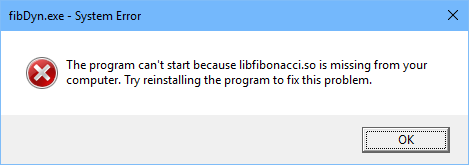
\includegraphics[scale=1]{../fibonacci/fibDynSystemError.png}
\caption{Windows error dialogue for missing library}
\end{figure}

































%CSparse
%Compiling
%All MingGW gcc commands (don't type the $ sign...)
%
% Copy the header file cs.h to Source and do "gcc -c *.o"
% Then in the same directory do "ar cr libcsparse.a *.o"
%
%Demo 1
%$ gcc ​-o cs_demo1 cs_demo1.c ./libcsparse.a -lm
%
%Demo 2
%First compile cs_demo to object-code (to get cs_demo.o) since it contains functions used by cs_demo2 and cs_demo3:
%
%$ gcc -c cs_demo.c -I../Include
%
%Now type:
%
%$ gcc -o cs_demo2 cs_demo.o cs_demo2.c -I../Include ../Source/libcsparse.a
%
%Demo 3
% As for cs_demo2
%

\begin{thebibliography}{1}

\bibitem{cinfree} Marcou, Engler and Varnek. {\em How to use C code in Free Pascal projects}. University of Strasbourg, 23 July 2009.

\end{thebibliography}

\end{document}
